\chapter{Research methodology} 

The research method used in this thesis follows the design science research (DSR) approach 
\cite[p. 17]{rennenkampff_managementitagilitaetentwicklung_2015}. 
DSR is a research paradigm in which the designer tries to create artifacts to answer questions for problems.

DSR is a research paradigm in which the designer creates artifacts and uses them to answer questions for problems and generate new scientific knowledge. 
The designed artifacts are both useful and fundamental to understanding the problem \cite[p. 10]{hevner_designscienceresearch_2010}

Design, according to Peffers et al. (2007), is the creation of an applicable solution to a problem \cite[p.47]{peffers_designscienceresearch_2007}

According to Hevner et al. (2010)
design" is both a process ("a set of activities") and a product ("artifactt"). \cite[p.78]{hevner_designscienceresearch_2010}
The design-oriented research approach as a methodological framework seems well suited to answer the research questions.
Predicting spring back and bend deduction is a relevant problem in business practice. 
Also, the conception and implementation of machine learning models is a design activity. 

The term artifacts is intentionally broad and can take on different forms. In this work, the artifact is different machine leaning models which are applied on the generated data. 
DSR can be implemented in various ways, a prominent example is provided by Peffers et al. and shown in Figure \ref{fig:dsr_process}
The approach comprises six steps, which are dived into the superordinate phases "Build" and "Evaluate". This thesis follows these phases.

 \begin{figure}
	\centering
	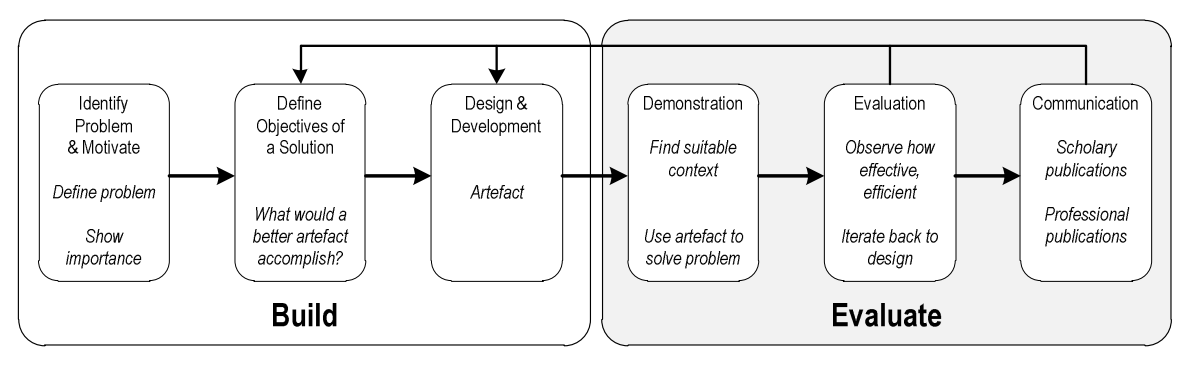
\includegraphics[width=1.1\linewidth]{chap3/images/dsr_process.png}
	\caption[DSR Process]{Design Science Research Approach according to Peffers et al. Picture: \cite[p. 72]{sonnenberg_evaluationpatternsdesign_2012}}
	\label{fig:dsr_process}
\end{figure}

\paragraph{Activity 1 - Problem identification and motivation} 
This activity includes defining a specific research problem and the value of a potential solution. 
The problem is used for the development of the artifact. To reduce complexity, the problem should be divided into sub-problems. For problem-solving, explicit methods such as system requirements gathering or an implicit method such as programming and/or data analysis. 
\cite[p. 52]{peffers_designscienceresearch_2007}

\paragraph{Activity 2: Define the objectives for a solution} 
The goals of a solution are derived from the problem definition. These are derived in the context of what is possible and feasible.
Objectives can be quantitative or qualitative. Objectives should be derived from the
problem specification and are thus based on the previous step. 
For knowledge about previous solutions and their effectiveness are required 
\cite[p. 55]{peffers_designscienceresearch_2007}

\paragraph{Activity 3: Design and development} 
This step involves the creation of the artifact. An artifact can potentially contain models,
methods or constructs, it can be anything that contributes to the solution of the research question. 
This step includes the definition of the functionality and architecture of the artifacts, followed by the creation of them.
\cite[p. 55]{peffers_designscienceresearch_2007}

\paragraph{Activity 4: Demonstration} 
The use of the previously created artifactt is demonstrated for one or more problems.
This requires effective knowledge of the artifact. 
\cite[p. 55]{peffers_designscienceresearch_2007}
% Descripe what is done in this work 

\paragraph{Activity 5 - Evaluation} 
It is observed and evaluated how well the developed artifact provides a solution to the defined problems in activity 1.
Knowledge of relevant metrics and methods of analysis is assumed. Depending on the nature of the problem, the evaluation can take different forms.
A comparison of the functionality of the artifact and other solutions can be considered. Furthermore, quantified
quantified parameters can be used to measure the performance of the artifacts
\cite[p. 56]{peffers_designscienceresearch_2007}
Hevner et al.  suggest five different evaluation methods: Observational
methods, analytical methods, experiments, testing of the artifact and descriptive
methods 
\cite[p. 87]{hevner_designscienceinformation_2004}
% How is this work evaluated 

\paragraph{Activity 6 - Communication} 
The problem and the artifactt and its benefit are communicated externally 
\cite[p. 56]{peffers_designscienceresearch_2007}
Hevner et al. describe in a conceptual framework guidelines for the

\section{Design Principles} 
Design Principles (DP) are seen as a central part of design-oriented research.
\cite[p. 348]{gregor_positioningpresentingdesign_2013}
Design principles are characterized as "principles of form and function" as well as "principles of implementation" of an artifact.
\cite[p.8]{gregor_anatomydesigntheory_}
They are used to close the gap between researchers and user and allow prescriptive research on systems. They are used to capture knowledge about the artifact. 
\cite[pp. 37-56]{sein_actiondesignresearch_2011}.
Koppenhagen et al. suggest generating design principles by grouping requirements for the solution and then creating core requirements, which can
which can then be DPs.
\cite[p. 6]{koppenhagen_designscienceresearch_2012}


\section{Evaluationn of Machine Learning Models }
tbd...

\subsection{Goal Question Metric Approach}
To make the defined quality attributes measurable, the “Goal-Question-Metric”-approach (GQM) was chosen in this work, which is one of the most common approaches and is divided into three levels: 
(Basili et al., 2002, p. 3).

\paragraph{1. conceptual level (goal):}
A goal, which usually corresponds to a quality criterion, is set for an object.
\paragraph{2. operational level (question):}
Questions are asked to define how an objective can be achieved.
\paragraph{3. quantitative level (metric):}
A set of data is associated with each question with the aim of answering it. Depending on the question, the data can be collected and evaluated objectively or subjectively.

Objectives, questions and metrics can be presented in a hierarchical structure.

\begin{figure}[ht!] % supposedly places it here ...
	\centering
	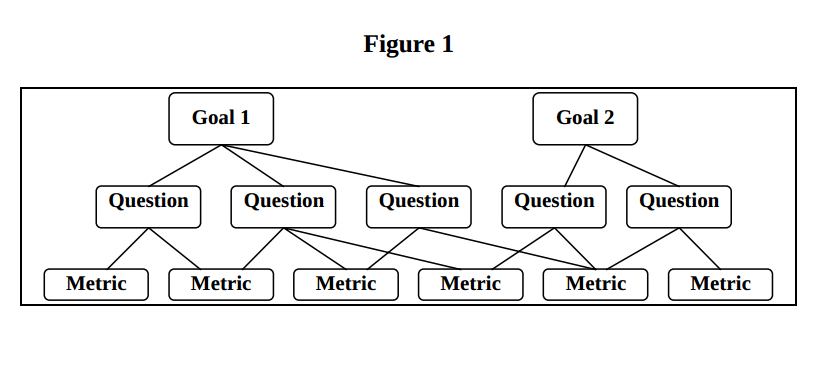
\includegraphics[width=0.6\linewidth]{gqm}
	\caption[GQM tree stucture ]{Goal-Question-Metric Ansatz \cite[p. 3]{basili_goalquestionmetric_}} 
	\label{fig:gqm}
\end{figure}




